\documentclass[conference]{IEEEtran}
\IEEEoverridecommandlockouts
\usepackage{cite}
\usepackage{amsmath,amssymb,amsfonts}
\usepackage{graphicx}
\usepackage{float}
\usepackage{textcomp}
\usepackage{xcolor}
\usepackage{booktabs}
\usepackage{tikz}
\usetikzlibrary{positioning,fit,backgrounds}

% ---------------------------------------------------------------------------
% DRAFT MARKER. \todo{} marks text that is NOT yet backed by evidence.
% Every one of these must be resolved or deleted before submission.
% Comment out the definition below to typeset a clean copy.
% ---------------------------------------------------------------------------
\newcommand{\todo}[1]{\textcolor{red}{\textbf{[TODO: #1]}}}

\begin{document}

\title{Waiting Is an Action: Event-Driven Time Primitives\\ for Long-Horizon GUI Agents}

\author{\IEEEauthorblockN{Saad Mujeeb}
\IEEEauthorblockA{\textit{University College of Engineering} \\
\textit{Osmania University}\\
Hyderabad, India \\
saifmujeeb2603@gmail.com}
}

\maketitle

\begin{abstract}
Graphical user interface (GUI) agents are evaluated almost exclusively on tasks
that complete within minutes, yet real desktop work is punctuated by waiting:
for a reply, a download, a build, or a person. We observe that current agent
architectures have no way to express duration. The ReAct loop models an agent as
a sequence of actions, so an agent that must wait can only emit repeated no-op
actions and re-examine the screen --- polling. When the poller is a language
model, each poll costs a full model round-trip, and the cost of waiting scales
with wall-clock duration. Browser automation solved this long ago with
event-driven primitives such as Playwright's \texttt{wait\_for\_selector}, but
those require a DOM; an agent that perceives only pixels has no equivalent. We
contribute the pixel-level analogue: waiting as a first-class action, with fixed
(\texttt{sleep}) and event-driven (\texttt{wait\_for\_screen\_change})
primitives evaluated server-side, outside the model loop. Event-driven waiting
reduces waiting from $O(T/p)$ model calls to $O(1)$ \emph{on a quiescent
screen}, degrading toward polling as screen activity rises --- a trade-off we
characterize rather than hide. Across a controlled experiment of four waiting
strategies over eight screens, event-driven waiting matches polling's
sub-10-second reaction at a median of $3$ model calls against polling's $7$ ---
as responsive as polling at under half the cost on a quiescent screen --- while
degrading to $5$--$6$ calls once on-screen noise crosses the detector's
threshold. Given both a fixed and an event-driven primitive under a neutral
prompt, the agent chose the event-driven one in $84\%$ of waits.
In a 19.1-hour, 63-run deployment, 32\% of active agent time was spent waiting,
which suggests the regime is not a corner case.
\end{abstract}

\begin{IEEEkeywords}
GUI agents, computer-use agents, vision-language models, long-horizon autonomy,
agent architectures, cost analysis
\end{IEEEkeywords}

% ===========================================================================
\section{Introduction}
\label{sec:intro}
% ===========================================================================

Consider an agent asked to watch for a colleague's reply and act on it. The
reply arrives in thirty minutes. The agent's actual work --- read the message,
draft an answer, send it --- takes four actions. The other thirty minutes are
spent doing nothing, and doing nothing is the expensive part.

This is not the regime that GUI agent research measures. Benchmarks such as
WindowsAgentArena~\cite{waa}, OSWorld~\cite{osworld}, and WebArena~\cite{webarena}
evaluate tasks that finish in minutes and score them on success rate. They report
neither wall-clock duration nor the token cost of waiting, because in their
regime waiting is negligible. In deployment it is not: in the 63-run deployment
we describe in Section~\ref{sec:eval}, waiting consumed 32\% of active agent
time.

\subsection{The gap}
The dominant agent architecture, ReAct~\cite{react}, models an agent as an
interleaved sequence of thoughts and actions. Time \emph{between} actions is not
modeled at all. An agent that must wait therefore has only one expressible
option: emit a short no-op action, receive a fresh observation, and decide again.
This is polling, and it has a cost model. For a wait of duration $T$ and poll
interval $p$, the agent makes
\begin{equation}
N_{\text{calls}} = \left\lceil T/p \right\rceil
\label{eq:poll}
\end{equation}
model calls, each returning a screenshot that is, by construction, almost always
identical to the last. The agent pays a model round-trip per poll to learn that
nothing has happened.

The critical detail is \emph{who} is polling. Polling versus event-driven waiting
is old ground in systems: \texttt{select}, \texttt{epoll}, and \texttt{inotify}
settled it decades ago, and browser automation frameworks such as
Playwright~\cite{playwright} and Selenium~\cite{selenium} have long exposed
event-driven waits like \texttt{wait\_for\_selector}. We claim no novelty in the
mechanism. What differs is the setting. A \texttt{select()} poll costs a syscall;
a poll in an agent loop costs a language model inference --- several orders of
magnitude more, in both money and latency. A cost that is ignorable at syscall
scale becomes the dominant term at model scale. Moreover, the browser-automation
solution does not transfer: \texttt{wait\_for\_selector} needs a DOM, and a
vision-language agent that perceives the screen as pixels has no DOM to query.
The primitive that solves this problem for browsers is unavailable to precisely
the agents that most need it.

\subsection{Insight and contributions}
Our insight is that \textbf{waiting is itself an action, and unlike other actions
it can be evaluated outside the model loop.} Nothing requires the model to be
present while time passes. If the waiting predicate is evaluated server-side and
the model is woken only when the predicate fires, the model call count decouples
from the duration.

We contribute:
\begin{itemize}
  \item \textbf{C1.} A characterization of three waiting strategies --- polling,
  fixed server-side (\texttt{sleep}), and event-driven
  (\texttt{wait\_for\_screen\_change}) --- and a pixel-level event-driven waiting
  primitive for agents without DOM access (Section~\ref{sec:waiting}).
  \item \textbf{C2.} An empirical cost--latency comparison of the three
  strategies, and a characterization of the change-detection threshold that
  governs the trade-off between false wakes and missed changes
  (Section~\ref{sec:eval}).
  \item \textbf{C3.} A design for agent-initiated human handoff, and
  observations from a 63-run, 19.1-hour deployment
  (Sections~\ref{sec:handoff} and~\ref{sec:eval}).
\end{itemize}

% ===========================================================================
\section{Related Work}
% ===========================================================================

\subsection{Computer-use agents}
Agents that operate a desktop or browser directly from pixels have progressed
rapidly, from Anthropic's computer-use reference implementation~\cite{anthropic}
to ScreenAgent~\cite{screenagent} and OpenHands~\cite{openhands}. These systems
establish the perception--action loop we build on. All are evaluated on
short-horizon tasks, and none model duration as a first-class quantity.

\subsection{Visual grounding}
A substantial line of work addresses translating semantic intent into screen
coordinates: OmniParser~\cite{omniparser} tokenizes screenshots into semantic
elements, Set-of-Mark~\cite{som} overlays numeric identifiers to let the model
select an ID rather than infer coordinates, and SeeClick~\cite{seeclick} trains
grounding directly. This work is orthogonal to ours. We use the normalized
coordinates the model emits natively and take no position on grounding; a better
grounder would improve our agent's actions without changing anything about how it
waits.

\subsection{Agent loops}
ReAct~\cite{react} established the observe--reason--act loop that most agents
implement, and subsequent work has extended it toward planning and reflection.
These architectures model the agent's \emph{steps}. None models the time between
them, which is the gap this paper addresses.

\subsection{Waiting in automation frameworks}
Browser automation has treated waiting as a first-class concern for years.
Playwright~\cite{playwright} and Selenium~\cite{selenium} provide explicit waits
(\texttt{wait\_for\_selector}, \texttt{WebDriverWait}) that block until a DOM
predicate holds, evaluated in the driver rather than the client. This is exactly
the right design, and it is the design we port. The obstacle is representational:
these predicates are expressed over the DOM. A vision-language agent observes a
rendered bitmap and has no queryable structure, so the predicate must be
expressed over pixels instead --- which introduces a false-wake regime that the
DOM formulation does not have, and which Section~\ref{sec:waiting} makes explicit.

\subsection{Benchmarks}
\label{sec:gap}
WindowsAgentArena~\cite{waa}, OSWorld~\cite{osworld}, WebArena~\cite{webarena},
and ScreenSpot~\cite{seeclick} are the standard evaluations for GUI agents. Each
reports task success rate. \emph{None reports wall-clock duration, and none
reports the token cost of waiting.} This is a reasonable omission for tasks that
complete in minutes, and it is precisely why the long-horizon cost regime remains
uncharacterized. Our work targets that gap.

% ===========================================================================
\section{System}
% ===========================================================================

We evaluate within a small agent runtime. \textbf{The runtime is not a
contribution of this paper} --- it follows established practice, and we describe
it only enough to make the measurements reproducible.

The system has three parts (Fig.~\ref{fig:arch}). A \emph{daemon} (Python, asyncio, HTTP on port 8420)
owns the task queue and exposes control endpoints. A \emph{brain} implements a
ReAct loop against the Gemini computer-use tool. A \emph{sandbox} (Docker, Xvfb,
openbox, \texttt{xdotool}, \texttt{scrot}) provides an isolated X11 desktop; this
recipe follows Anthropic's reference implementation~\cite{anthropic}.

One design property is load-bearing later: \textbf{screenshots are captured on
demand, one per decision, not streamed.} The agent's perception is a discrete
sequence of frames requested at action boundaries. Consequently an agent that
wants to know whether the screen has changed must \emph{ask}, and asking is a
model round-trip. This is what makes polling expensive, and it is a property of
every screenshot-based agent architecture we are aware of, not an artifact of our
implementation.

\begin{figure}[t]
\centering
\resizebox{\columnwidth}{!}{%
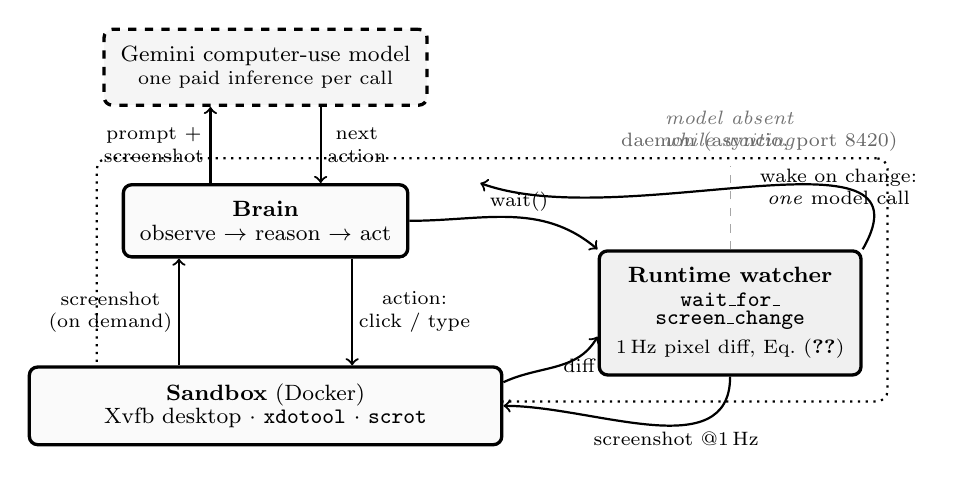
\begin{tikzpicture}[
  font=\footnotesize,
  comp/.style={rounded corners=3pt, draw, very thick, align=center,
               inner sep=6pt, minimum height=9mm},
  ext/.style={comp, dashed, fill=black!4},
  watch/.style={comp, fill=black!6},
  el/.style={font=\scriptsize, align=center, inner sep=2pt},
  ar/.style={-{>}, thick},
]
% --- components ---------------------------------------------------------
\node[ext] (gem) at (0,4.3)
     {Gemini computer-use model\\[-1pt]\scriptsize one paid inference per call};
\node[comp, fill=black!2, minimum width=34mm] (brain) at (0,2.35)
     {\textbf{Brain}\\[-1pt]observe $\to$ reason $\to$ act};
\node[comp, fill=black!2, minimum width=60mm] (sand) at (0,0)
     {\textbf{Sandbox} (Docker)\\[-1pt]Xvfb desktop $\cdot$ \texttt{xdotool} $\cdot$ \texttt{scrot}};
\node[watch, minimum width=30mm, align=center] (w) at (5.9,1.18)
     {\textbf{Runtime watcher}\\[-1pt]\texttt{wait\_for\_}\\[-3pt]\texttt{screen\_change}\\[1pt]
      \scriptsize 1\,Hz pixel diff, Eq.~(\ref{eq:change})};

% --- decision loop (a model call every step): sand -> brain -> gem -> act
\draw[ar] ([xshift=-7mm]brain.north) -- node[el,left]{prompt {+}\\screenshot}
          ([xshift=-7mm]gem.south);
\draw[ar] ([xshift=7mm]gem.south)  -- node[el,right]{next\\action}
          ([xshift=7mm]brain.north);
\draw[ar] ([xshift=-11mm]sand.north) -- node[el,left]{screenshot\\(on demand)}
          ([xshift=-11mm]brain.south);
\draw[ar] ([xshift=11mm]brain.south) -- node[el,right]{action:\\click / type}
          ([xshift=11mm]sand.north);

% --- wait loop (no model call): brain hands off, watcher diffs frames ----
\draw[ar] (brain.east) to[out=0,in=140]
          node[el,above,pos=.55]{wait()} (w.north west);
\draw[ar] (w.south) to[out=-90,in=0]
          node[el,below,pos=.4]{screenshot @1\,Hz} (sand.east);
\draw[ar] (sand.east) ++(0,3mm) to[out=25,in=-120]
          node[el,right,pos=.5]{diff} ([yshift=-3mm]w.west);
\draw[ar] (w.north east) to[out=60,in=-20]
          node[el,right,pos=.5]{wake on change:\\\emph{one} model call} ([xshift=9mm]brain.east|-brain.north);

% the model is idle during the wait: state it, since it is the whole point
\node[el, text=black!55, align=center] at (5.9,3.5)
     {\emph{model absent}\\\emph{while waiting}};
\draw[dashed, black!35] (w.north) -- (5.9,3.05);

% --- component groupings (daemon owns queue + watcher; brain is its worker)
\begin{scope}[on background layer]
  \node[draw, dotted, thick, rounded corners, fit=(brain)(w),
        inner sep=9pt, label={[el,text=black!60]above right:daemon (asyncio, port 8420)}] {};
\end{scope}
\end{tikzpicture}%
}
\caption{System architecture. The \emph{decision} loop (left, solid) spends one
Gemini inference per step: the sandbox returns a screenshot on demand, the brain
reasons and emits an action. The \emph{wait} loop (right) is the contribution:
the brain hands off to a runtime watcher that diffs $1$\,Hz screenshots against a
baseline (Eq.~\ref{eq:change}) and re-enters the model exactly once, with one
fresh frame, when the screen changes. \textbf{No model call occurs while time
passes.} Screenshots are captured per decision, never streamed, which is why
polling---re-asking the model whether anything changed---costs a full round-trip
each time.}
\label{fig:arch}
\end{figure}

% ===========================================================================
\section{Waiting as a First-Class Action}
\label{sec:waiting}
% ===========================================================================

We expose three waiting strategies to the model and characterize each.

\subsection{Polling baseline (\texttt{wait})}
The model emits a short fixed wait, receives a fresh screenshot, and re-decides.
Cost follows~(\ref{eq:poll}): $N_{\text{calls}} = \lceil T/p \rceil$. Reaction
latency is bounded by $p$. No prior knowledge of $T$ is required, which is why
models reach for it. This is the strategy an agent falls into by default when the
architecture gives it no way to say ``wait.''

\subsection{Fixed server-side waiting (\texttt{sleep})}
The model emits one call specifying a duration; the runtime sleeps up to 3600\,s
outside the model loop and returns a single fresh screenshot.
$N_{\text{calls}} = 1$, independent of $T$. The cost is that $T$ must be known in
advance: overshoot wastes wall-clock, undershoot fails the wait.

One interaction is worth recording because it is a trap. A long sleep must extend
the task's own deadline, or waiting kills the task it was meant to enable. We
push the deadline out by the sleep duration plus a margin
(\texttt{SLEEP\_DEADLINE\_MARGIN} $=60$\,s). An implementation that omits this
turns a working \texttt{sleep} primitive into a timeout bug.

\subsection{Event-driven waiting (\texttt{wait\_for\_screen\_change})}
The model blocks until the screen visibly changes, with no round-trips while
waiting. The runtime captures a baseline frame, then compares against it at
1\,Hz, returning on the first frame that differs.

Frames are compared as $240\times152$ grayscale thumbnails. A pixel counts as
changed if it shifts by more than $\delta = 14$ (of 255); a frame counts as
changed if more than $\phi = 0.004$ (0.4\%) of its pixels changed:
\begin{equation}
\text{changed}(a,b) = \mathbb{1}\!\left[\;\left|\{\,i : |a_i - b_i| > \delta\,\}\right|
> \phi \cdot |a|\;\right]
\label{eq:change}
\end{equation}
The thresholds are set to be eager: a single new chat bubble should trip the
detector, while a blinking caret or a moved mouse cursor (a few pixels) should
not. Section~\ref{sec:rq2} characterizes them empirically rather than asserting
they are correct.

% Algorithm box, hand-formatted: the algorithm/algorithmic packages are not
% dependencies, so this compiles on a bare TeX Live install.
\newcommand{\algline}[2]{\makebox[1.8em][r]{\footnotesize #1:}\hspace{0.4em}#2\\}
\newcommand{\algind}{\hspace*{1.2em}}
\begin{figure}[t]
\hrule\vspace{2pt}
\textbf{Algorithm 1} Event-driven wait, evaluated server-side
\vspace{2pt}\hrule\vspace{4pt}
{\footnotesize\ttfamily\raggedright
\algline{}{\textbf{Input:} timeout $T_{\max}$, sandbox $S$}
\algline{}{\textbf{Output:} (changed, elapsed)}
\algline{1}{$b \leftarrow$ Thumbnail(Screenshot($S$))}
\algline{2}{$t_0 \leftarrow$ MonotonicNow() \hfill $\triangleright$ not wall-clock; \S\ref{sec:setup}}
\algline{3}{\textbf{while} MonotonicNow() $- \; t_0 < T_{\max}$ \textbf{do}}
\algline{4}{\algind \textbf{if} Cancelled() \textbf{or} WakeRequested() \textbf{then}}
\algline{5}{\algind\algind \textbf{return} (false, MonotonicNow() $-\; t_0$)}
\algline{6}{\algind \textbf{end if}}
\algline{7}{\algind $f \leftarrow$ Thumbnail(Screenshot($S$))}
\algline{8}{\algind \textbf{if} Changed($b$, $f$) \textbf{then} \hfill $\triangleright$ Eq.~(\ref{eq:change})}
\algline{9}{\algind\algind \textbf{return} (true, MonotonicNow() $-\; t_0$)}
\algline{10}{\algind \textbf{end if}}
\algline{11}{\algind Sleep(1s) \hfill $\triangleright$ no model call here}
\algline{12}{\textbf{end while}}
\algline{13}{\textbf{return} (false, $T_{\max}$)}
}
\vspace{2pt}\hrule
\label{alg:wait}
\end{figure}

Crucially, the loop in Algorithm~\ref{alg:wait} contains no model call. The model
is absent while time passes and is re-entered exactly once, with one fresh
screenshot, when the predicate fires.

\subsection{Cost analysis}
\label{sec:cost}
Table~\ref{tab:strategies} summarizes the three strategies.

\begin{table}[t]
\caption{Waiting strategies. $T$ is wait duration, $p$ poll interval,
$F$ false wakes.}
\label{tab:strategies}
\centering
\small
\begin{tabular}{@{}lccc@{}}
\toprule
 & \textbf{poll} & \textbf{\texttt{sleep}} & \textbf{event-driven} \\
\midrule
Model calls        & $\lceil T/p \rceil$ & $1$        & $1 + F$ \\
Reaction latency   & $\leq p$            & $\leq T$   & $\leq 1$\,s \\
Needs $T$ upfront  & no                  & yes        & no \\
Server compute     & $O(1)$              & $O(1)$     & $O(T)$ diffs \\
\bottomrule
\end{tabular}
\end{table}

Two honest qualifications follow, both of which a careful reviewer would raise.

\paragraph{$O(1)$ is conditional, not unconditional}
Event-driven waiting costs $1 + F$ model calls, where $F$ counts wakes on changes
irrelevant to the agent's goal. $F$ is not a constant. On a quiescent screen
$F \approx 0$ and the cost is genuinely $O(1)$. But on a screen with periodic
activity --- a ticking clock, an animated spinner, an unrelated notification ---
false wakes arrive at some rate $r$, giving $F \approx rT$ and a cost of $O(rT)$.
In the limit of continuous motion (video playback), event-driven waiting fires
every frame and \emph{collapses into polling, but worse}: every wake is a full
model call, with no interval $p$ to bound the rate. The correct statement of our
claim is therefore: \textbf{$O(1)$ model calls on a quiescent screen, degrading
toward polling as screen activity rises.} Section~\ref{sec:rq2} measures where
that boundary lies; it is the central trade-off of the design, not a footnote.

\paragraph{Prompt caching complicates the token model}
Equation~(\ref{eq:poll}) counts \emph{model calls}, and that count is exact.
Translating it into \emph{tokens} is not straightforward, because providers
implicitly cache repeated prompt prefixes, so successive polls may bill less than
their nominal prompt size. The precise claims are: (i) model calls remain
$\lceil T/p \rceil$ --- caching does not remove round-trips; (ii) each call still
pays its uncached delta, which includes the new screenshot, the expensive part;
and (iii) each call still pays its full latency. We therefore instrument and
report cached and uncached prompt tokens separately, and treat \textbf{model
calls and latency as primary metrics}, since neither can be deflated by caching.
Under the RQ1 workload, implicit caching does materialize but only partially:
$19\%$ of the polling arm's prompt tokens were billed as cached, rising to
$24$--$35\%$ for the arms with fewer, more varied calls. Caching therefore
discounts the token bill without removing the round-trips or the per-call
screenshot, consistent with claims (i)--(iii) above.

% ===========================================================================
\section{Evaluation}
\label{sec:eval}
% ===========================================================================

The three research questions are all backed by data: \S\ref{sec:rq1} the
cost--latency experiment, \S\ref{sec:rq2} the threshold sweep, and
\S\ref{sec:rq3} the deployment observations.

\subsection{Setup}
\label{sec:setup}
\textbf{Task suite.} Eight synthetic waiting scenes with known ground truth, in
three groups. Three are \emph{quiescent}: a dialog that appears after a delay, a
terminal build that prints a completion line, and a download whose banner is
replaced on completion. Four form a \emph{noise ladder}: the same wait against
increasing background activity (a spinner, a small and a large ticking clock, a
scrolling log), whose amplitudes are \emph{measured} against the detector
threshold rather than judged by eye and span from below it to well above it
(\S\ref{sec:rq2}). One is a \emph{no-change control} that never resolves, to
measure timeout cost and catch hallucination. Every event reveals a codeword the
agent must echo back, so a run that never watched the screen cannot score as a
success. The driver fires each event at a fixed point on the monotonic clock, so
reaction latency is a subtraction, not an inference.

\textbf{Conditions.} Four arms --- poll, \texttt{sleep}, event-driven, and a
free-choice arm exposing both \texttt{sleep} and event-driven described neutrally
--- each leaving the model exactly one way to express a wait (the free arm, two),
so that any difference is architectural rather than a prompting effect. The
prompt never names a strategy; the available primitive is set by ablating the
toolbox. Four arms $\times$ eight scenes $\times$ five repeats $=160$ runs.

\textbf{Metrics.} Model calls; prompt tokens, reported as cached and uncached
separately; output tokens; reaction latency (ground-truth change $\rightarrow$
first agent action); and task wall-clock.

\textbf{Measurement of duration.} All durations are recorded with an in-process
monotonic clock, never as differences of wall-clock timestamps. This is not
pedantry. In our deployment logs (\S\ref{sec:rq3}), host suspend inflated
wall-clock spans by 22 hours across 63 runs --- 54\% of the naive total --- while
in-process durations were unaffected. A wait that reports 19\,s of elapsed loop
time may span 10 hours of wall-clock if the host sleeps in between. \emph{On a
suspendable host, wall-clock deltas are not durations.} Experiments are run on a
host with suspend disabled.

\subsection{RQ1: cost versus latency across strategies}
\label{sec:rq1}

The prediction, registered in advance, was: polling achieves low latency at
$O(T/p)$ calls; \texttt{sleep} achieves $O(1)$ calls but latency proportional to
overshoot; event-driven achieves both on quiescent screens and degrades as noise
rises. Table~\ref{tab:rq1} and Fig.~\ref{fig:rq1} bear this out.

\begin{table}[t]
\caption{RQ1 per-strategy cost, latency, and success. Medians across the eight
scenes; model calls and reaction latency are the primary metrics
(\S\ref{sec:cost}).}
\label{tab:rq1}
\centering
\small
\begin{tabular}{@{}lccc@{}}
\toprule
 & \textbf{model calls} & \textbf{reaction (s)} & \textbf{success} \\
\midrule
poll               & 7 & 8.6  & 100\% \\
\texttt{sleep}     & 3 & 45.7 & 100\% \\
event-driven       & 3 & 7.8  & 97\%  \\
free choice        & 3 & 8.3  & 94\%  \\
\bottomrule
\end{tabular}
\end{table}

\begin{figure}[t]
\centering
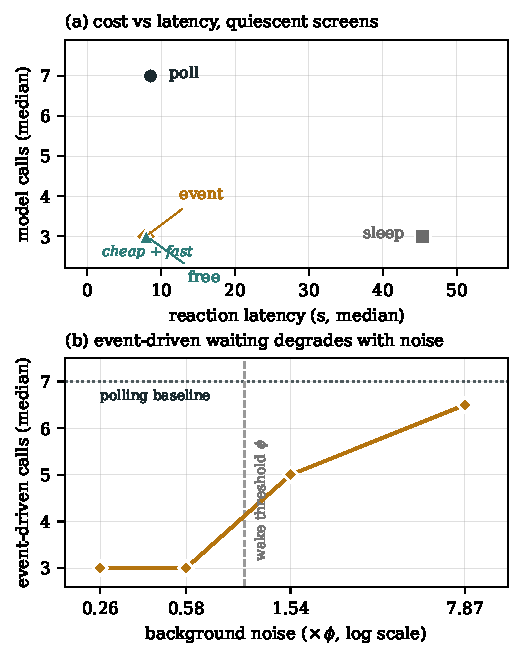
\includegraphics[width=\columnwidth]{fig2}
\caption{RQ1. \textbf{(a)} On quiescent screens, event-driven and free-choice
waiting occupy the cheap-and-fast corner: polling's $\leq$10\,s reaction at a
third of \texttt{sleep}'s latency and under half of polling's model calls.
\textbf{(b)} The event-driven arm's cost as background noise sweeps across the
detector threshold $\phi$: flat at the $O(1)$ floor while noise sits below
$\phi$, rising toward the polling baseline above it --- the predicted
$O(1)\!\to\!O(rT)$ transition, located between $0.58\times$ and $1.54\times\phi$.}
\label{fig:rq1}
\end{figure}

\textbf{Cost and latency.} Polling spends a median of $7$ model calls per wait;
\texttt{sleep}, event-driven, and free-choice each spend $3$. Reaction latency
separates them the other way: polling and event-driven both react in under
$9$\,s, while \texttt{sleep} reacts in $45.7$\,s --- the overshoot of a fixed
guess. Event-driven waiting thus lands where the cost model predicted, matching
polling's responsiveness at less than half its model calls
(Fig.~\ref{fig:rq1}a).

\textbf{Degradation with noise.} Fig.~\ref{fig:rq1}b sweeps the event-driven arm
across the noise ladder. Below the detector threshold ($0.26\times$ and
$0.58\times\phi$) it holds the $O(1)$ floor of $3$ calls, indistinguishable from
a still screen: motion that \emph{looks} busy but stays under $\phi$ costs
nothing. Above the threshold it degrades --- $5$ calls at $1.54\times$, $6$ at
$7.87\times$ --- climbing toward polling's $7$ exactly as $O(1)\!\to\!O(rT)$
predicts. The transition sits where the ladder crosses $\phi$, confirming the
threshold governs the trade-off rather than merely bounding it.

\textbf{What the reaction number contains.} Reaction latency is end-to-end
(ground-truth change $\rightarrow$ first agent action) and therefore folds in one
Gemini round-trip, not just detection. Decomposing the event-driven runs, the
\emph{detection} component (change $\rightarrow$ the watcher waking) has a median
of $2.1$\,s --- near the $1$\,Hz sampling bound --- while the model round-trip
that follows adds a median of $5.4$\,s, for $7.5$\,s end-to-end. The model term
is a fixed cost of consulting a language model and is shared across all arms, so
it inflates the absolute numbers without biasing the comparison; the architecture
controls only the $2.1$\,s detection term, which is where event-driven waiting
wins.

\textbf{The one miss.} Polling and \texttt{sleep} never fail; event-driven and
free-choice succeed $97\%$ and $94\%$ of the time. The rare miss is the eager
detector's failure mode --- a wake on incidental motion that the model acts on
before the true event, or a below-threshold signal --- and is the price of the
$O(1)$ cost, not a contradiction of it.

\subsection{RQ2: change-threshold characterization}
\label{sec:rq2}

The threshold $\phi$ trades false wakes against missed changes. To locate that
boundary we captured $1$\,Hz frame streams from three noise scenes and the signal
transition, then replayed the production wake loop (Algorithm~\ref{alg:wait})
offline at every $\phi$ --- counting false wakes on the noise and testing whether
the real event still trips the detector. Fig.~\ref{fig:rq2} shows the result.

\begin{figure}[t]
\centering
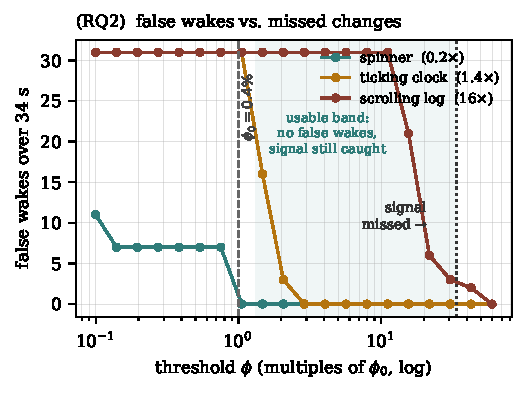
\includegraphics[width=\columnwidth]{fig3}
\caption{RQ2. False wakes over a $34$\,s window as the threshold $\phi$ sweeps
(log scale, in multiples of the production $\phi_0 = 0.4\%$), for three noise
scenes; the dotted line marks the signal amplitude, above which the real event is
missed. The spinner ($0.2\times\phi_0$) never trips $\phi_0$; the ticking clock
($1.4\times$) and scrolling log ($16\times$) do, and only stop as $\phi$ is
raised past their amplitude. The signal sits at $33.6\times\phi_0$, leaving a wide
usable band in which no noise wakes the detector yet the event is still caught.}
\label{fig:rq2}
\end{figure}

Two things follow. First, the false-wake curves fall to zero exactly as $\phi$
passes each scene's measured amplitude ($0.2\times$, $1.4\times$, $16\times\phi_0$),
confirming that $\phi$ \emph{governs} the $O(1)\!\to\!O(rT)$ boundary of
\S\ref{sec:cost} rather than merely bounding it: a scene is quiescent-in-effect
precisely when its amplitude sits below $\phi$. Second, the signal changes
$33.6\times\phi_0$ of the screen --- far above every noise scene --- so any $\phi$
in the band $[\,1.4\times,\,33.6\times\,]\phi_0$ eliminates the clock's false
wakes while still catching the event. The production $\phi_0$ sits at the eager
end of the safe range: it admits some false wakes on the busier scenes (which the
model filters, \S\ref{sec:waiting}) in exchange for never missing a signal, the
asymmetry we intended. Raising $\phi$ toward the signal amplitude would trade
those false wakes for missed events on any scene whose real signal is smaller
than the banner used here --- the reason we do not, and the reason a fixed scalar
$\phi$ is a floor for future work rather than the final answer.

\subsection{RQ3: deployment observations}
\label{sec:rq3}
We report descriptive statistics from 63 runs of the system during development
and personal use.

\textbf{This data is observational, not experimental}, and we draw no causal
conclusions from it. Runs pursued heterogeneous goals (web research, media
playback, messaging, shell introspection); there were no controls, no repeats,
and no hypothesis fixed in advance. Its role here is solely to establish that the
waiting regime occurs in practice.

\begin{table}[t]
\caption{Deployment observations, 63 runs. Durations are in-process
monotonic measurements; see \S\ref{sec:setup}.}
\label{tab:deploy}
\centering
\small
\begin{tabular}{@{}lr@{}}
\toprule
Runs & 63 \\
Active agent time (suspend-free) & 19.1\,h \\
Total actions & 3{,}893 \\
\midrule
Time spent inside waits & 6.1\,h (32\% of active) \\
\texttt{wait\_for\_screen\_change} calls & 359 \\
\quad ended in a detected change & 240 \\
\quad ended by operator wake & 19 \\
\quad timed out with no change & 100 \\
\texttt{sleep} calls & 7 \\
Polling \texttt{wait} calls & 354 \\
\bottomrule
\end{tabular}
\end{table}

The load-bearing observation in Table~\ref{tab:deploy} is that \textbf{32\% of
active agent time was spent waiting}. Waiting is not a corner case in deployment
even though it is absent from benchmarks (\S\ref{sec:gap}).

We explicitly decline to interpret the 359-to-7 ratio of event-driven to fixed
waits as evidence of a preference. The tool descriptions presented to the model
recommend \texttt{wait\_for\_screen\_change} over \texttt{sleep}; the ratio
therefore measures instruction-following, not a discovered property. To separate
the two we ran the free-choice arm of \S\ref{sec:rq1}, which exposes both
primitives described neutrally, with no recommendation. There the agent still
chose event-driven waiting in $84\%$ of waits ($59$ of $70$), and free-choice
matched the event-driven arm on cost and latency (Table~\ref{tab:rq1}). The
preference survives removal of the prompt bias, though under a single model we
claim it no further.

% ===========================================================================
\section{Agent-Initiated Human Handoff}
\label{sec:handoff}
% ===========================================================================

Some waits cannot be resolved by waiting: a login, a captcha, a decision only a
human can make. We treat these as a distinct primitive rather than a failure.

\texttt{wait\_for\_user} lets the agent declare itself blocked, state what it
needs, and suspend; the operator acts, and the agent resumes with a fresh
screenshot. A complementary guard escalates automatically: three consecutive
empty or filtered model responses trigger a handoff rather than an unbounded
retry loop. The operator may also inject \emph{guidance} mid-run without
restarting the task.

Across the deployment we observed 17 agent-initiated handoffs (logins, a captcha,
a credential entry) and 203 operator guidance messages. We present these as
design and qualitative observation only: there is no controlled baseline, and the
203 guidance messages indicate a human was frequently in the loop --- these runs
were supervised, not autonomous, and should not be read as evidence of unattended
operation.

% ===========================================================================
\section{Limitations and Ethics}
% ===========================================================================

\textbf{The degenerate case.} On a screen with continuous motion, event-driven
waiting fires on every frame and performs \emph{worse} than polling, since each
false wake is an unbounded-rate model call (\S\ref{sec:cost}). Our primitive is
correct only for screens that are quiescent between meaningful events. We regard
naming this regime as a precondition for claiming the other one.

\textbf{Pixel-level detection is blind to off-screen change.} A download that
completes without updating the display will not wake the agent; this is precisely
where \texttt{sleep} remains necessary, and why we retain all three strategies
rather than proposing one.

\textbf{Scope.} A single model, a single desktop environment, a single worker,
and one screen resolution. The thresholds in~(\ref{eq:change}) are tuned for this
configuration and we make no claim that they transfer.

\textbf{Observational data.} Section~\ref{sec:rq3} is descriptive. Goals differed
across runs and none were repeated; it establishes that a regime exists, nothing
more.

\textbf{Ethics.} The agent executes exclusively inside a Docker-isolated
sandbox with no host filesystem access. Our deployment logs contain third-party
conversation data --- messages from people who did not consent to appearing in a
research artifact. \todo{Decision required before any artifact release: scrub
\texttt{runs/} of all third-party content, or withhold the logs and release only
the code and the synthetic task suite. The motivating example opening
Section~\ref{sec:intro} is synthetic for this reason. Do not release the raw
logs.}

% ===========================================================================
\section{Conclusion}
% ===========================================================================

Waiting is an action. Agent architectures that model only steps force waiting to
be expressed as polling, and when the poller is a language model, polling makes
the cost of doing nothing scale with the duration of doing nothing. Moving the
waiting predicate server-side decouples model calls from wall-clock time --- on a
quiescent screen, and with a false-wake term that grows as that assumption
weakens. The trade-off is the contribution; the primitive is the easy part.

% ===========================================================================

% ===========================================================================
\begin{thebibliography}{00}

% ---------------------------------------------------------------------------
% \todo{EVERY entry below must be verified against the actual publication
% before submission: authors, venue, year, page numbers. Do not submit a
% citation you have not personally opened. Target 25--35 refs; this is a
% starting skeleton, not a finished bibliography.}
% ---------------------------------------------------------------------------

\bibitem{react} S. Yao, J. Zhao, D. Yu, N. Du, I. Shafran, K. Narasimhan, and
Y. Cao, ``ReAct: Synergizing reasoning and acting in language models,'' in
\emph{Proc. Int. Conf. Learning Representations (ICLR)}, 2023.

\bibitem{waa} R. Bonatti \emph{et al.}, ``Windows Agent Arena: Evaluating
multi-modal OS agents at scale,'' \emph{arXiv:2409.08264}, 2024.

\bibitem{osworld} T. Xie \emph{et al.}, ``OSWorld: Benchmarking multimodal agents
for open-ended tasks in real computer environments,'' in \emph{Advances in Neural
Information Processing Systems (NeurIPS)}, 2024.

\bibitem{webarena} S. Zhou \emph{et al.}, ``WebArena: A realistic web environment
for building autonomous agents,'' in \emph{Proc. Int. Conf. Learning
Representations (ICLR)}, 2024.

\bibitem{omniparser} Y. Lu, J. Yang, Y. Shen, and A. Awadallah, ``OmniParser for
pure vision based GUI agent,'' \emph{arXiv:2408.00203}, 2024.

\bibitem{som} J. Yang, H. Zhang, F. Li, X. Zou, C. Li, and J. Gao, ``Set-of-Mark
prompting unleashes extraordinary visual grounding in GPT-4V,''
\emph{arXiv:2310.11441}, 2023.

\bibitem{seeclick} K. Cheng, Q. Sun, Y. Chu, F. Xu, Y. Li, J. Zhang, and Z. Wu,
``SeeClick: Harnessing GUI grounding for advanced visual GUI agents,'' in
\emph{Proc. Annu. Meeting Assoc. Computational Linguistics (ACL)}, 2024.

\bibitem{screenagent} R. Niu \emph{et al.}, ``ScreenAgent: A vision language
model-driven computer control agent,'' in \emph{Proc. Int. Joint Conf. Artificial
Intelligence (IJCAI)}, 2024.

\bibitem{openhands} X. Wang \emph{et al.}, ``OpenHands: An open platform for AI
software developers as generalist agents,'' in \emph{Proc. Int. Conf. Learning
Representations (ICLR)}, 2025.

\bibitem{anthropic} Anthropic, ``Computer use (beta) --- reference
implementation,'' 2024. [Online]. Available:
https://docs.anthropic.com/en/docs/build-with-claude/computer-use

\bibitem{playwright} Microsoft, ``Playwright: Auto-waiting and web assertions,''
2024. [Online]. Available: https://playwright.dev/docs/actionability

\bibitem{selenium} Selenium Project, ``Waits --- Selenium documentation,'' 2024.
[Online]. Available: https://www.selenium.dev/documentation/webdriver/waits/

\end{thebibliography}

\end{document}
